
%%%%%%%%%%%%%%%%%%%%%%% file typeinst.tex %%%%%%%%%%%%%%%%%%%%%%%%%
%
% This is the LaTeX source for the instructions to authors using
% the LaTeX document class 'llncs.cls' for contributions to
% the Lecture Notes in Computer Sciences series.
% http://www.springer.com/lncs       Springer Heidelberg 2006/05/04
%
% It may be used as a template for your own input - copy it
% to a new file with a new name and use it as the basis
% for your article.
%
% NB: the document class 'llncs' has its own and detailed documentation, see
% ftp://ftp.springer.de/data/pubftp/pub/tex/latex/llncs/latex2e/llncsdoc.pdf
%
%%%%%%%%%%%%%%%%%%%%%%%%%%%%%%%%%%%%%%%%%%%%%%%%%%%%%%%%%%%%%%%%%%%


\documentclass[runningheads,a4paper]{llncs}

\usepackage{amssymb}
\setcounter{tocdepth}{3}
\usepackage{graphicx}

\usepackage{url}
\urldef{\mailsa}\path|{alfred.hofmann, ursula.barth, ingrid.haas, frank.holzwarth,|
\urldef{\mailsb}\path|anna.kramer, leonie.kunz, christine.reiss, nicole.sator,|
\urldef{\mailsc}\path|erika.siebert-cole, peter.strasser, lncs}@springer.com|    
\newcommand{\keywords}[1]{\par\addvspace\baselineskip
\noindent\keywordname\enspace\ignorespaces#1}

\begin{document}

\mainmatter  % start of an individual contribution

% first the title is needed
\title{Cloud-SAT-Solver based on obfuscating CNF}

% a short form should be given in case it is too long for the running head
\titlerunning{Lecture Notes in Computer Science: Authors' Instructions}

% the name(s) of the author(s) follow(s) next
%
% NB: Chinese authors should write their first names(s) in front of
% their surnames. This ensures that the names appear correctly in
% the running heads and the author index.
%
\author{Ying Qin%
\thanks{Please note that the LNCS Editorial assumes that all authors have used
the western naming convention, with given names preceding surnames. This determines
the structure of the names in the running heads and the author index.}%
\and ShengYu Shen\and Yan Jia\and QingBo Wu\and HuaDong Dai}
%
\authorrunning{Lecture Notes in Computer Science: Authors' Instructions}
% (feature abused for this document to repeat the title also on left hand pages)

% the affiliations are given next; don't give your e-mail address
% unless you accept that it will be published
\institute{Springer-Verlag, Computer Science Editorial,\\
Tiergartenstr. 17, 69121 Heidelberg, Germany\\
\mailsa\\
\mailsb\\
\mailsc\\
\url{http://www.springer.com/lncs}}

%
% NB: a more complex sample for affiliations and the mapping to the
% corresponding authors can be found in the file "llncs.dem"
% (search for the string "\mainmatter" where a contribution starts).
% "llncs.dem" accompanies the document class "llncs.cls".
%

\toctitle{Lecture Notes in Computer Science}
\tocauthor{Authors' Instructions}
\maketitle


\begin{abstract}
Propositional satisfiability (SAT) has been widely used in hardware and software verification. With the emerging cloud computing paradigm, it becomes increasingly motivated to outsource complex SAT problem to the commercial public cloud for larger computation demand and greater flexibility. But outsourcing SAT solving to cloud also bring in new security challenge, that is, some confidential information encoded in CNF formula may be leaked to unauthorized third party.
In this paper, we propose a novel cloud-oriented SAT solving algorithm to preserve privacy. First,an obfuscated CNF formula is generated by embedding a Husk formula into the original CNF. formula with proper rules; Second, the obfuscated CNF formula is solved by a state-of-the-art SAT solver deployed in cloud; Third, a simple mapping algorithm is used to map the solution of the obfuscated formula back to that of the original CNF formula. Theoretical analysis demonstrates that, this obfuscating algorithm can significantly change the structural characteristics of original CNF formula, while keeping its solution space unchanged. Theoretical analysis and experimental result shows that the obfuscating algorithm and mapping algorithms are all with linear complexity.
\emph{abstract} environment.
\keywords{SAT-solver; CNF formula; Privacy; obfuscate; cloud-computing}
\end{abstract}


\section{Introduction}

Propositional satisfiability [1] (SAT) has been widely used in hardware and software verification [2][3]. With the rapid increase of the hardware and software system, the size of SAT problem generated from verification also increases rapidly. 
On the other hand, cloud computing paradigm can provide elastic computing resource to meet the workload demand of different application. It becomes increasingly motivated to outsource complex SAT solving procedure from local sites to the commercial public cloud [35][37]. However, when outsourcing SAT solving,computing data shall be send into remote server which is shared among different client. Threat of information leakage resulted from authorized access to outsourcing data make an obstacle to widely adopt the new computing paradigm. 
In formal verification, circuit, code and property will be converted into CNF (Conjunctive Normal Form) formula through Tsentin[4] coding before SAT solving. After Tsentin encoded, circuit structure and other sensitive information are still existed in CNF formula. To prevent unauthorized user get sensitive information from CNF formula, obfuscating CNF formula becomes necessary.
This paper presents a novel Cloud-SAT-solver based on Obfuscating CNF. First, the original CNF formula S1 is obfuscated into a new CNF formula S, by embedded through proper rules with a CNF formula S2 which has unique solution, embedding rules guarantee S has different graph structure compared with S1; second, S is sent to SAT-solver S which deployed in Cloud, S generates Solution of G and send it back; third, the solution F is obtained from the solution of G by projection, the correctness is guaranteed by embedding rules in first step.
The advantage of this method is that: firstly, through obfuscation, sensitive information in original CNF formula, such as circuit structure, will not be available in Obfuscated CNF formula which is outsourced into cloud; secondly, Obfuscated CNF formula can be solved by SAT solver without any modification. Finally, the theoretical analysis and experiments shows that obfuscating and solution recovery algorithms linear complexity, reducing the impact on the overall performance of SAT solving.
In the following sections: Chapter II describes the background; Chapter III gives the description of the problem; Chapter IV gives the implementation of cloud-SAT-solver based on obfuscation; Chapter V analyzes correctness, effectiveness and algorithm complexity of the obfuscation algorithm; Chapter VI describes the related work; Chapter VI gives the experimental results; Chapter VII summarizes.

\section{Background}
\subsection{Preliminaries}

A problem handled by SAT solver is usually specified in a conjunctive normal form (CNF) formula of propositional logic. A CNF formula is represented using Boolean variables that can take the values 0 (false) or 1 (true). Clauses are disjunction of literals, which are either a variable or its complement, and a CNF formula is a conjunction of clauses.
φ=(x1∨¬x2)∧(x2∨x3)∧(x2∨¬x4)∧(¬x1∨¬x3∨x4 )
φ is a typical example of CNF formula, which contains four variables x1, x2, x3, x4, and four clauses x1∨¬ x2, x2∨x3, x2∨¬x4, ¬x1∨¬ x3∨x4. In clause x1∨¬ x2, there are two literals x1 and ¬x2. literal x1 is called positive literal of variable x1.while ¬x2 is called negative literal of variable x2.
The number of literals in clause C is length of C, denoted as |C|.For example | x1∨¬x2|2
Solving SAT problem is to determine if there exists an assignment to the variables of CNF formula such that the formula can be satisfied. CNF formula is satisfied (SAT) if and only if each clause in the CNF formula takes value 1, that means at least one literal in the clause takes value 1.If there does not exist assignment to the variables such that the formula can be satisfied, CNF formula is UNSAT, whereas Clauses which is conflicted with each other is called unsatisfied core.

\subsection{Tseitin coding}

In hardware verification, Circuits and property are converted into CNF formula through Tseitin coding[4],then CNF formula is handled by SAT solver. 
Every circuit can be expressed by combination of gate AND2 and NOT, so here lists Tseitin coding of them. 
For gate AND2 z=NOT(x), its CNF formula generated by Tseitin encoding, is  (x∨z) ∧(¬x∨¬z).
While for gate AND2 z=AND2(x1,x2), its CNF formula is (¬x1∨¬x2∨z)∧(x1∨¬z) ∧(x2∨¬z).
For other type gate, its according CNF formula can be generated through Tseitin encoding.
For a complex circuit consists of basic gate, such as AND2和NOT, the CNF formula of the circuit is conjunctive of formulas of basic gate.
As illustrated in Fig. 1, Fig 1a) circuit consists of a gate of AND and a gate of OR. Through Tseitin encoding, CNF formula of 1a) circuit  is expressed as conjunctive of clauses in Fig .1b) and Fig .1c).
\begin{figure}
\centering
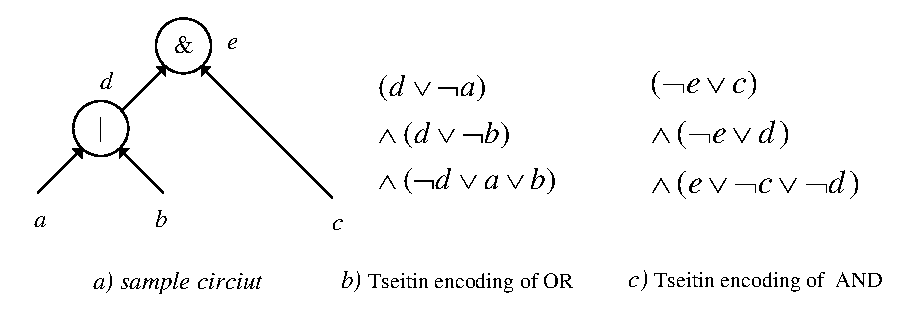
\includegraphics[width=9.2cm]{a1}
\caption{Tseitin form of circuit $x_s$ (\emph{dotted kernel}) or two kernels at
$x_i$ and $x_j$ (\textit{left and right}) lead to the same summed estimate
at $x_s$. This shows a figure consisting of different types of
lines. Elements of the figure described in the caption should be set in
italics, in parentheses, as shown in this sample caption.}
\label{fig:example}
\end{figure}
Formally, for any circuit C, it can be converted into CNF formula φ through Tseitin, note as φ=Tseitin(C).
This paper focuses on obfuscation of CNF formula generated from circuit in formal verification, the obfuscation algorithm is also suitable for CNF formula generated from software code.

\section{Problem Definition}

\subsection{Model of SAT solving in cloud}

In cloud computind paradigm, there is three step involved in verification oriented SAT solving, as illustrated in Fig. 2
\begin{figure}
\centering
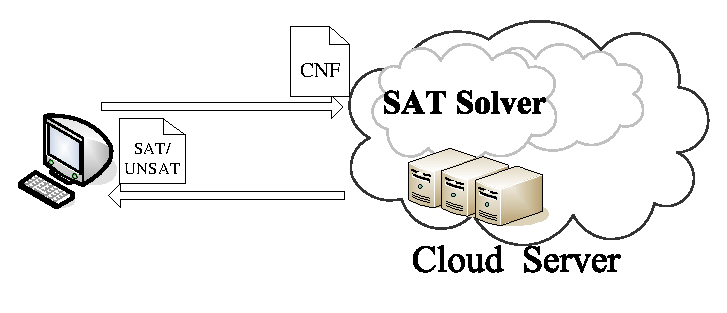
\includegraphics[width=9.2cm]{a2}
\caption{SAT solving in cloud $x_s$ (\emph{dotted kernel}) or two kernels at
$x_i$ and $x_j$ (\textit{left and right}) lead to the same summed estimate
at $x_s$. This shows a figure consisting of different types of
lines. Elements of the figure described in the caption should be set in
italics, in parentheses, as shown in this sample caption.}
\label{fig:example}
\end{figure}
1) Upload computing data:User converts circuit into CNF formula and upload to cloud server through client.
\newline 2)  SAT solve: SAT solver deployed in cloud server handles CNF formula, and gives solution.If CNF formula is SAT, solver will give an assignment of the variables; While if CNF formula is UNSAT, solver will give an unsatisfied core.{}
\newline 3)  Download solution: User get solution from cloud through client.{}

\subsection{Threat Model}
In cloud computing paradigm, CNF formula will be uploaded and handled in public cloud; Cloud are multi-tenant, unauthorized access[11] to CNF formula may result in leakage of sensitive information.
\newline On the other hand,result verification of SAT problem is simple: if CNF formula is SAT, just check if CNF formula is satisfied under the assignment given by cloud; while if CNF formula is UNSAT, just get unsatisfied core from cloud. Result verifications for both conditions are all linear complexity.
\newline According to facts listed above, in this paper,we assume that cloud computing servers are honest but curious: cloud servers will complete the SAT solving tasks correctly, but CNF formula may be analyzed to obtain additional information, such as all or part of the circuit structure.
\newline The information of circuit structure is not lost during encoding from circuit to CNF. Li [6] and Ostrowski [7] discuss the techniques to extract circuit structures from CNF formula. Furthmore , Roy [8] and Fu [9]  present algorithm of CNF-to-circuit decoding to recover circuit structure from CNF formula.
\newline Before we discuss the algorithm of CNF-to-circuit decoding, concepts in algorithms are introduced first.  
\newline Definition 1. A CNF-signature of a logic gate is a CNF formula representing the characteristic function of the gate. Clause in CNF-signature is called characteristic clause. If a characteristic clause contains all variables in CNF-signature, the clause is named key clause. Variable represents Output of a logical gate is called output variable.
\newline Take gate AND as an example, after Tseitin coding , three input AND gate (AND3) is converted into the set of clauses C as shown in figure 3.

\begin{figure}
\centering
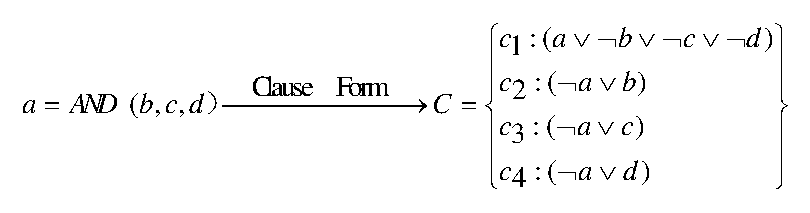
\includegraphics[width=9.2cm]{a3}
\caption{Fig 3 CNF signature of gate AND3  $x_s$ (\emph{dotted kernel}) or two kernels at
$x_i$ and $x_j$ (\textit{left and right}) lead to the same summed estimate
at $x_s$. This shows a figure consisting of different types of
lines. Elements of the figure described in the caption should be set in
italics, in parentheses, as shown in this sample caption.}
\label{fig:example}
\end{figure}

C is a CNF signature of gate AND3. c1~c4 is characteristic clause of gate AND3. Clause c1 that contains all the variables in gate AND3, is key clause. a is the output variable.
\newline Under encoding rules, gate with the same characteristics function will be encoded into the same set of clauses. Potential attackers can exploit structural knowledge from CNF Formulas to restore the circuit structure. Some restoring circuit structure algorithms are based on concept of directed hyper-graph and bipartite graph.	

Definition 5 (Hypergraph of CNF)
\newline Let Σ be a CNF formula. A graph of clauses G = (V, E) is associated to Σ s.t.
\newline each vertex of V corresponds to a clause of  Σ;
\newline each edge (c1 , c2 ) of E corresponds to a variable of Σ, while c1 c2 contain the same variable or complement.
\newline each edge is labeled by the variable.
 
Definition 6 (Directed Hypergraph of CNF)
\newline Let Σ be a CNF formula. A graph of clauses G = (V, E) is associated to Σ s.t.
\newline – each vertex of V corresponds to a clause of Σ;
\newline – each edge (c1 , c2 ) of E corresponds to a variable of Σ, while c1 c2 contain the same variable ;
\newline – Endpoint of edge is labeled by + (when clause contains variable ) or -(when clause contains complement of variable).

Definition 7 (bipartite of CNF)
\newline Let Σ be a CNF formula. A graph of clauses G = (V, E) is associated to Σ s.t.
\newline – each vertex of V corresponds to clause and variable of Σ;
\newline – each edge (c , v ) of E corresponds to a pair of clauses c and variable v of Σ, while c contains v ;
\newline – each edge is labeled by + (when clause contains variable ) or -(when clause contains complement of variable).

Fig.4a) gives the corresponding Hyper-Graph of gate AND3 in Fig.3. 
Fig.4c) gives the corresponding Directed Hyper-Graph of gate AND3 in Fig.3. while | represents positive, - represents negative variable.
Fig.4b) gives the corresponding Bipartite Graph of gate AND3 in Fig.3.
\begin{figure}
\centering
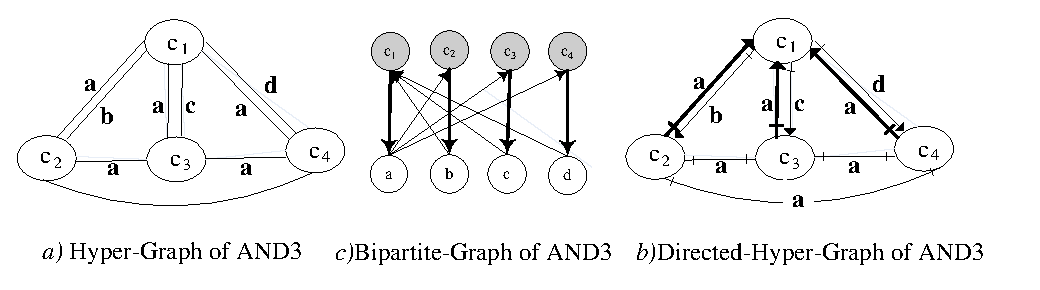
\includegraphics[width=9.2cm]{a4}
\caption{Graph representation of gate AND3}
\label{fig:example}
\end{figure}

Based on definitions list above, Roy, etc.[8] articulats that an arbitrary combinational circuit can be encoded as a CNF-SAT instance so that its circuit structure is preserved and can readily be extracted. they describe algorithms for restoring circuit structure from CNF formulas and empirically show its success and scalability on very large benchmarks. The basic steps in their Generic Circuit Detection algorithm are as follows 
\newline 1)	Convert the CNF instance to an undirected graph
\newline 2)	Convert the CNF signature of the gate to match to an undirected graph
\newline 3)	Use subgraph isomorphism to match instances of the gate
\newline 4)	To piece together the circuit, create a maximal independent set (MIS) instance ,one node per detected gate an edge between nodes if the gates are incompatible,(signatures overlap, etc.)

Fu[9] presents a tool CNF2CKT to implement CNF-to-circuit decoding. The CNF2CKT algorithm effciently extracts a maximum circuit structure from any given CNF instance. Some important features of CNF2CKT are:
\newline 1) It uses generic pattern matching techniques to detect all possible gate matchings (candidate matchings) for every logic gate in a user-specified gate library.
\newline 2) It then constructs a maximum acyclic combinational circuit by selecting a maximum subset of gate matchings, i.e. a cover, from all the candidate matchings. Maximum here is with respect to the number of logic gates in the extracted circuit, i.e. the size of the cover, since one matching corresponds to one logic gate in the extracted circuit. The cover is maximum in the sense that no other circuit structure containing more logic gates can be extracted from the CNF description.

These circuit structure extraction algorithms are based on subgraph isomorphism and pattern matching, exploiting the graph structure characteristics of CNF formula. In cloud computing paradigm,threats can use these algorithms to obtain the circuit structure information carried by CNF formula. Therefore, It is essential to prevent information leakage when outsourcing CNF formula to cloud.

\section{Cloud-SAT-solver with privacy-preserving}

In this paper, we present a Cloud-SAT-solver based on obfuscating algorithm, which prevent information leakage through hiding the structure in CNF formula. The Obfuscating algorithm is based on three facts and anticipation: First, since CNF signature is key in circuit extraction, altering CNF signature of gate in CNF formula will make circuit extraction algortigm losing efficacy. Second, the current classical SAT solver [10] is efficient with integration of mechanisms such as conflict detection,Unit propergation. Distinct from obfuscating algorithm in literature[11] which develops a brand-new SAT-solving algorithm, we wish to take advantage of classical SAT solver.Last,we anticipate the solution of obfuscating CNF formula may be much easily mapped into original CNF formula.
\newline The proposed algorithm is also dependent on the following definition.

Definition 8: Husk formula is a CNF formula with a unique solution,in which assignment of variables is non-specific(Not all 0 or all 1).
\newline The procedure of Cloud SAT-solver based on obfuscating algorithm is shown in Fig.7
\begin{figure}
\centering
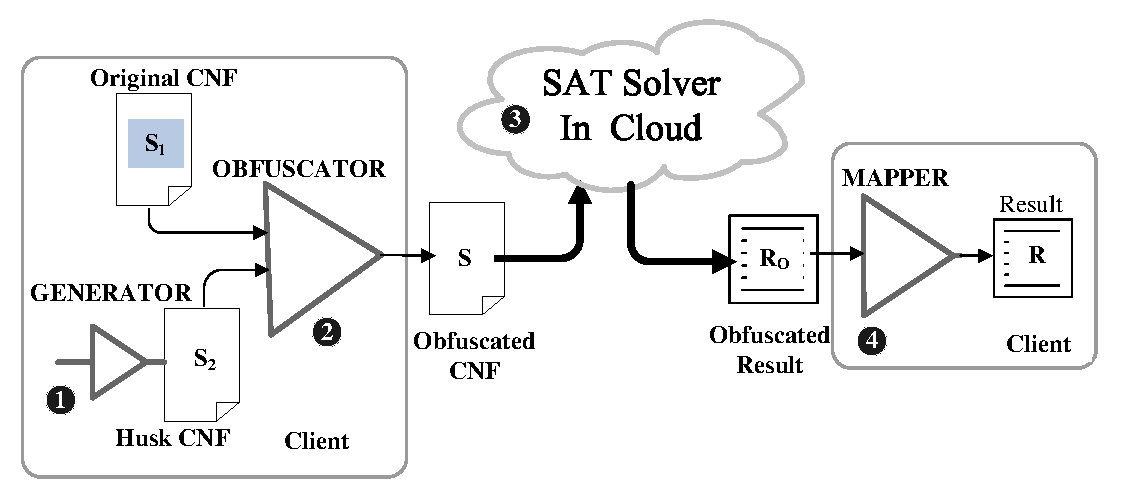
\includegraphics[width=10.2cm]{a5}
\caption{procedure of Cloud SAT-solver based on obfuscating CNF $x_s$ (\emph{dotted kernel}) or two kernels at
$x_i$ and $x_j$ (\textit{left and right}) lead to the same summed estimate
at $x_s$. This shows a figure consisting of different types of
lines. Elements of the figure described in the caption should be set in
italics, in parentheses, as shown in this sample caption.}
\label{fig:example}
\end{figure}

The main steps of the algorithm are listed in the table below, except step 3 is on the cloud server, the remaining steps 1, 2 and 4 is done locally.

Procedure of Cloud SAT-solver based on obfuscatin algorithm
\newline input:original CNF formula S1 
\newline output:solution of original CNF formula S1
\newline 1 GENERATOR generates a Husk formula with a unique solution Hr.
\newline 2 OBFUSCATOR obfuscates S1 with S2 and Hr , obtains a new CNF formula S。
\newline 3 Outsource S to cloud server, where SAT solver solves it and outputs its solution. 
\newline 4 Mapper receives solution of S from cloud, and recovers solution of S1 from that of S 

It need be emphasized that, S1 and S2 have disjoint set of variables. In subsequent sections 4.1, 4.2 and 4.3,the generator, obfuscator and mapper will be described in detail. 

\subsection{generate Husk formula}
From the point of view of cryptology, Husk formula is a secret key used to encrypt the CNF formula. Our obfuscating algorithm requires Husk formula has a unique solution. In this paper, Husk formula is constructed based on prime factorization method: given prime X with a binary vector representation X = <x1,x2…,xn>, taking square of X as the of the output of multiplier M, while banning X equals 1. Then converting the multiplier M into CNF formulaφ. Through construction above, the two inputs of M must all be X = <x1,x2…,xn>,can CNF formula of M be satisfied. That means assignment of input variable is unique . Since assignment of all variables in CNF formula of M are decided by assignment of inputs variable.So,φ has a unique solution. Assuming multiplier M (I1, I2, O), in which there are two inputs I1 and I2, and one output O.GENERTOR algorithm to generate Husk formula is listed below.

Algorithm of GENERTOR
\newline Input:NULL
\newline Output:Husk CNF S2,Husk result Hr
\newline 1:generate a prime number p
\newline 2:  sq=p*p
\newline 3:φ=M(I1≠1, I2≠1, O=sq)
\newline 4:  S2=Tseitin(φ)
\newline 5:  Hr=p|p

\subsection{construct obfuscating formula}

The proposed obfuscating algorithm is to generates a new CNF formula S, by embedding clauses and variables(as literal) of Husk formula S2 into Original formula S1 with proper rules ,(there is no intersection between variables set of S2 and S1). Through adding new clauses and new literals, the algorithm alters the clause set and literal set in clauses of S1,so as to obfuscating CNF signature in S1. Proper rules guarantees solution space is invariant, that means, S and S1 can be solved with the same SAT-solver. There is following relationship between solutions of S and that of S1: S is unsatisfied iff S1 is unsatisfied; S is satisfied iff S1 is satisfied, and solutions of S1 can be extracted from solutions of S by projection on variables set of S1.Details of implementation is in OBUFSCATOR algoritms.

OBFUSCATOR算法

In order to keep solution space invariant, when insert variable of S2 into clauses of S1 , rules must be followed (OBFUSCATOR algorithm,line 6、20): variables,which is assigned F in Hr (unique solution of S2),are as positive literals; variables,which is assigned T in Hr (unique solution of S2),are as negtive literals. Rationality of the rules will be explained in section 4.1

In algorithm(lines 1-3 , line 7-12), there is macro Algorithm2 . When the macro is defined, $“mark”$ (line 2) and $“generate-new-clause”$ (line 9) . Procedure $“mark”$ marks key clauses and output variables of some kind of gate in CNF formula. Procedure $“generate_new_clause”$ generates some new clauses matching the key clauses, so as to  assemble new CNF signature( such as assemble CNF-signature of AND3 based that of AND2, details presented in section 5.2), therefore improve the hardness of distinguish gates.

Gate of different type has different forms in key clauses and output variable, such that different mark algorithms are needed ,but complexity of these mark algorithms is of the same. Here take AND2 gate as example ,detailed implementation is presented in AND2MARK algoritm.  
AND2MARK算法

Same as mark algorithm, Here take AND2 gate as example ,,details are in GENAND2CLAUSE algoritm.
GENAND2CLAUSE算法

$“mark”$ algorithm need to analyze structure in CNF formula, times to run is up to number of clauses and variables in CNF formula.Since,Obfuscator runs in client, such as panel or PC.Whether to use mark algorithm or not is depended on computation capabity of client.

Inserting positive/negative literal into clause or appending new clause into formula will result in the transformation of key clause and CNF signature in formula, therefore bringing corresponding changes in hypergraph and bipartite-graph of CNF formula.These transformations reflect the effectiveness of obfuscation. The algorithm presented here trys to attain three goals: first, transforming the original key clause and CNF-signature of gates in CNF formula partly; second, transforming key clause and CNF-signature of same type gate into different forms; third, make length of each clause in formula are equal as far as possible. Achieving goal 1 and 3 is able to prevent formula from structure detection through pattern matching techniques. While achieving goal 2 is able to prevent formula from structure detection through subgraph isomorphism techniques. 

\subsection{Recover the original solution}
The variables in S is superset of that in S1.In obfuscating algorithm, Mapping table M is used to map variable name from S1 to S. Therefore, to get solution of S1 ,we need filter assignment of variables in S1 from Or according to the variable name mapping table M. Or is the solution of S,given by SAT-solver located in the cloud. Procedure to get solution of S1 is implemented by MAPPER algorithm.
MAPPER算法

\section{Correctness,effectiveness and performance analysis}
The obfuscating, algorithm blends the original formula seamless with Husk formula, correctness and effectiveness are basic requirements of the algorithm. 

The Correctness means that the algorithm should keep the solution space of the original CNF formula, that is, for CNF formulas S1 and its according obfuscated formula S, the following facts are hold: If S1 is unsatisfied, S is unsatisfied either, vice versa, and the unsatisfied core of S1 can be obtained by deleting literal in S2  from clauses in unsatisfied core of S; If S1 is satisfied, S is satisfied too, vice versa, and the solution of S1 can be obtained by projecting solution of S into variables of S1. 

The effectiveness of the algorithm refers to that changes brought to the CNF formula by obfuscating, make the circuit structure extraction work more difficult, or circuit structures can not be extracted anymore. 

Obfuscating algorithm and solution recovery algorithms are required to run on the client with weak computing power, algorithmic complexity should not be too high.

\subsection{Correctness analysis}
For illustration, OBFUSCATOR algorithm is simplified as follows. Since step 4 only remaps variable name, which will not affect assignment of variable, it will be ignored when discussed correctness.
\newline Step1. For each clause in S1 , take one or more variables in S2, insert them into clauses in S1, abiding by rule : if assignment of variable is T in Hr, insert negative literal of variable into clause; if assignment of variable is F in Hr, insert positive literal of variable into clause. New clauses generated by Step 1 constitutes clause set S3.
\newline Step2. (optional) generate new clause with literals in Hr and output variables in S1, abiding by rule : if assignment of variable is T in Hr, insert positive literal of variable into clause; if assignment of variable is F in Hr, insert negative literal of variable into clause. Literal forms of output variable is up to the key clause to which the output variable belongs. New clauses generated by step2 constitutes clause set S4.
\newline Step3. combine clauses in S2,S3,S4 (optional), disorder clauses and produce new formula S.
\newline Step4. remap variables name, and log mapping information into table M 

For illustration, the following definitions and settings are given.

Define 9. Variable in original CNF formula is called original variable; Clause in original CNF formula is called original clause. Variable in Husk formula is called Husk variable. Clause in Husk formula is called Husk clause. Literal constitutes result of Husk formula is called Husk literal.
\newline Orignal variable	X={x1,x2,…,xm}
\newline Orignal Sulotion	O={(a1,a2,…,am)×(x1,x2,…,xm) | ai∈ {T,F}}
\newline Husk variable  	Y={y1,y2,…,yn }
\newline Husk solution	        H={(b1,b2,…,bn)×(y1,y2,…,yn) | bi∈ {T,F}}
\newline Husk result	        Hr={(b1,b2,…,bn)×(y1,y2,…,yn)| bi∈ {T,F}}

According to algorithm ( step 3 in Table) listed above, there are two type of variables in obfuscated formula: original variable and Husk variable. While there are three type of clauses in obfuscated formula: Husk clause(clauses in S2),original clause blended with Husk variable( clauses in S3), clauses consist of Husk literal and output variable (clauses in S4) .

As we know, Husk formula is a unique solution, when GENERATOR generate Husk formula S2, it also give the result Hr={b1,b2,…,bm}. When assign Hr to variable, each clause in S2 will be T.

According to step 1 in algorithm, each clause in S3 can be expressed in form C=A∨B, while A is clause from S1, B= Bi, Bi=zi∨Bi-1, B1= z1.
\newline if bj==F, then zi =yi
\newline if bi ==T, then zi =¬yi

Under constrains of Husk clause,Husk variable must be assigned H={b1,b2,…,bm}, then zi must be F. So B=Bi= zi∨zi -1∨…∨z1 must be F. That means C= A∨B,Value of C is total up to A. So solution space of S3 is same as that of S1. For illustration,take a example.

Hypothesis: clause A and clause with unique variable B=b,while b is not variable in A。
let S1=A S2=B , Hr={(T)×(b) }
Obfuscating procedure:
\newline Step 1. according to Hr and rules ,get clause C=A∨¬b。let S3=C
\newline Step 2. (option)omit
\newline Step 3. let S= S2∧S3 ,then S=B∧C
\newline Step 4. omit
\newline prove:
\newline  ∵ S=B∧C  B=b      ∴ S=b∧C   
\newline  ∵ S=b∧C  C=A∨¬b  ∴ S=A∧b  
\newline  ∵ S=b∧A  B=b      ∴ S=B∧A
\newline  ∴ S=B∧A  S1=A S2=B ∴ S= S1∧S2

S4子句是由Husk解文字和原关键子句中的输出变量组成的子句,S4中的子句C都是形如C= zi∨A。其中:bi==F,则zi =¬yi 且bi ==T,则zi =yi。
\newline 受Husk子句的约束,Husk变量必须取值Hr={b1,b2,…,bm},因此zi=T,C= zi∨A=T,因此子句C不会对A中变量赋值的产生约束。举一个简单的例子来说明。

Hypothesis: clause A=a∨X and clause with unique literal B=b,while b is not variable in X。
\newline let S1=A S2=B then Hr ={(T)×(b) } 
\newline Obfuscating procedure:
\newline Step1、according to Hr and rule ,get子句C=A∨¬b,let S3=C
\newline Step2、according to Hr and rule ,take b as literal,take literal a in clause A,get clause D=a∨b, let S4 =D
\newline Step3、let S= S2∧S3∧S4,得到S=B∧C∧D
\newline Step4、omit
证明:
∵ S=B∧C∧D  B=b     ∴ S=b∧C∧D
∵ S=b∧C∧D  C=A∨¬b ∴ S=b∧(A∨¬b)∧D= b∧A∧D
∵ S=b∧A∧D  D=a∨b  ∴ S=b∧(a∨b)∧A= b∧A
∵ S=b∧A     B=b      ∴ S= B∧A 
∵ S=B∧A    S1=A  S2=B   ∴ S= S1∧S2

In conclusion, obfuscated formula S is equivalent to S1∧S2,assuming O, H, Z is solution of formula S1,S2,Z 
O={(a1,a2,…,am)×(x1,x2,…,xm) }, H={(b1,b2,…,bn)×(y1,y2…,yn)}, Z=O|H={(a1,a2,…,am,b1,b2,…,bn)×(x1,x2,…,xm,y1,y2,…,yn )}.
Under the obfuscating algorithm in this paper, the following theorem holds.
Theorem 1: S1, S2, S is CNF formula, S2 has only a unique solution, S = OBFUSCATOR (S1, S2); X is solution of S1, and Y is the solution of S2. Z is solution of S, then Z = X | Y,.
Theorem 2: S1, S2, S is CNF formula, S2 has only a unique solution, S = OBFUSCATOR (S1, S2); Z is solution of S, and Y is the solution of S2, then X = MAPPER (Z, S1.) is solution of S1.
Theorem 3: S1, S2, S is CNF formula, S2 has only a unique solution, S = OBFUSCATOR (S1, S2), S1 is unsatisfied, if and only if S is unsatisfied.
These theorems ensure the correctness of the obfuscating algorithm, solution space before and after obfuscating did not change. Appendix 1 gives a formal proof of these theorems.
\subsection{Effectiveness analysis}
As discussed in chapter 2, in the threat model, analysis of hyper-graph and bipartite graph is mean to extract circuit structure. In order to verify the effectiveness of the algorithm, we give the qualitative and quantitative analysis of changes to hyper-graph and bipartite graph brought by obfuscating.
\subsubsection{Qualitative analysis}
Assume there are instances a and e of gate AND2. Fig 6 give CNF signature and hyper-graph of a and e.
\begin{figure}
\centering
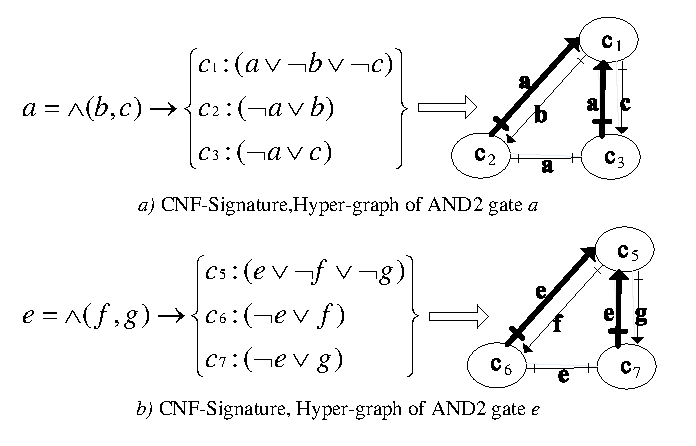
\includegraphics[width=9.2cm]{a6}
\caption{CNF-signature and Hyper-Graph of AND2 gate a and e}
\label{fig:example}
\end{figure}
Assume Husk result is {(F,F,F,F,T,F,T,T)×(A、B、C、D、E、F、G、H)}, after obfuscating, CNF signature and hypergraph of a and e are shown in Fig 9.
\begin{figure}
\centering
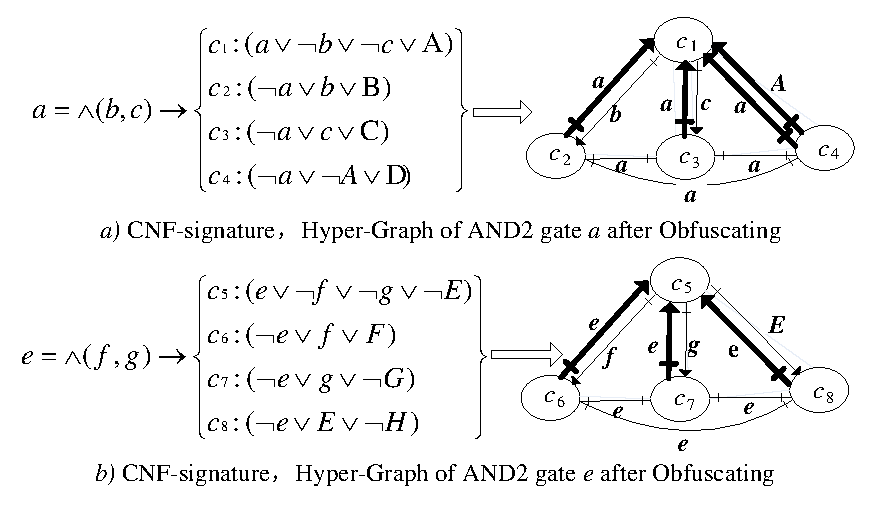
\includegraphics[width=9.2cm]{a7}
\caption{CNF-signature and Hyper-Graph of AND2 gate a and e after obfuscating}
\label{fig:example}
\end{figure}
Both a and e are instances of gate AND2. Changes to CNF signatures of a and e by obfuscating result in four effects. First, the length of c1 and c5, key clauses of a and e, is changed from 3 to 4, this change disables technique of key clause based pattern match presented in literature [9]. Second, after obfuscating, CNF-signature of a and e are different, thus hyper-graph of them are not isomorphic anymore, this change disables technique based on sub-graph isomorphic presented in literature [8]. Third, there are new clauses added in formula, such as c4 in a and c8 in e, this change disable structure detection techniques based on sub-graph matching. 
Furthermore, by inserting proper literal in key clauses and generating new clause, CNF signature of instance e is changed from AND2 to AND3, shown in Fig 9b), Husk variable E, which becomes a input variable of gate AND3, is indistinguishable with f and g ,which are original input variables of AND2.
Bipartite graphs of a and e, before and after obfuscating, are shown in fig.8 and fig.9.
\begin{figure}
\centering
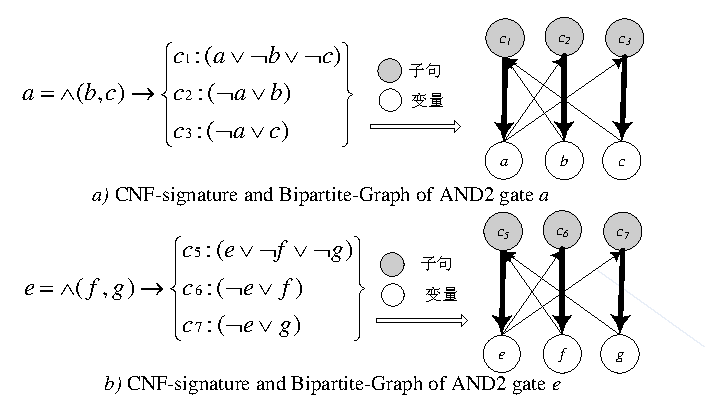
\includegraphics[width=9.2cm]{a8}
\caption{Bipartite-Graphs of AND2 gate a and e}
\label{fig:example}
\end{figure}
Obfuscating brings changes to bipartite graphs of a and e, furthermore, bipartite graph of them are not isomorphic anymore.
\begin{figure}
\centering
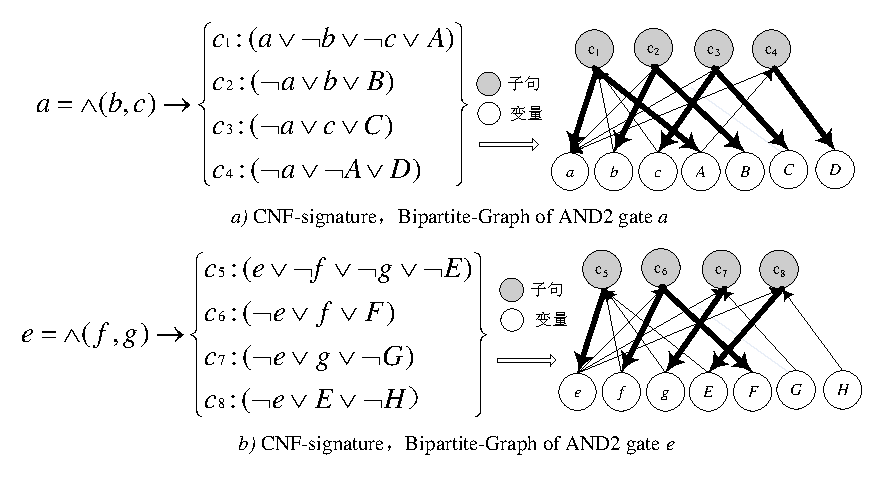
\includegraphics[width=9.2cm]{a9}
\caption{Bipartite-Graphs of AND2 gate a and e after obfuscating}
\label{fig:example}
\end{figure}
Analysis presented above only think about condition of inserting one variable into each clause, inserting more than one variable with different combination will bring more changes. 

\subsubsection{Quantitative analysis} 
Pattern matching and sub-graph isomorphism is means to detect gate structures in CNF formula. Since key clause or CNF signature oriented pattern matching is dependent on key clause and CNF signature, changing them could prevent such attacks. Through searching isomorphic sub-graph, the gate structure with same CNF signature can be detected; thus even modifying the CNF signature of instances, if instances of same type gate have the same new CNF signature, these instances can still be identified as the same type of gate through sub-graph isomorphism matching. After careful analysis, the orignal CNF signature may even be inferred. 

Therefore there are three level to measure changes to the CNF formula. The first level is to change key clause and characteristic clauses shown in 9a) and 10a); the second level is to change isomorphic relationship between CNF signature of instances, as shown in 10a) and 10b); the third level is to change CNF signature into distinguishable, that is, even detecting the same CNF signature, one is still unable to determine that two instances of the same CNF signature are corresponding to the same type of gate before obfuscating, as shown in Fig.9b) the instance of gateAND2 after obfuscating are distinguishable with instance of gate AND3 as shown in Fig5.
To measure the effectiveness, the following definitions are given.
Definition 10: If using pattern matching technique can not detect instances of a type of gate in a CNF formulas, CNF formula is called for such gate pattern matching attack safe, GPMA-safe.
Definition 11: If In a CNF formula, some instances of the same type of gate are not isomorphic, the CNF formula is called for such gate partially isomorphic attack safe, GPIA-safe; If In a CNF formula, any two instances of the same type gate are not isomorphic, the CNF formula is called for such gate completely isomorphic attack safe, GCIA-safe.
Definition 12: If in a CNF formula, same CNF signature may not be corresponds to same type of gate, the CNF formula is called for such gate structural safe, GS-safe.
Definition 13: If in a CNF formula, any type of gate is GPMA-safe, the CNF formula is called pattern matching attack safe, PMA-safe.
Definition 14: If in a CNF formula , there exists a type of gate which is GPIA-safe, the CNF formula is called PIA-safe; If in a CNF formula, every type of gate are GCIA-safe, the CNF formula is called CIA-safe.
Definition 15 : If in a CNF formula, any type of gate is GS-safe , the CNF formula is called S-safe.
Transforming a CNF formula into PMA-safe will increase the difficulty to recover circuit structure; while transforming a CNF formula into PIA-safe can prevent complete circuit structure from detection; futhermore  transforming a CNF formula into S-safe can prevent any part of circuit structure from detection.
Definition 16: If there are n characteristic clauses in CNF signature of a certain type of gate, insert m literals into each clauses, distinguished between positive or negative literal,the maximum number of new CNF signature for this gate can be derived is  .When the number of instances is more than T, according to the drawer principle, there must be 2 or more instances have the same new CNF signature, thus through sub-graph isomorphic searching, one can detect gates which has same CNF signature. z is Called isomorphic threshold.

For example, gate AND2 consists three characteristic clauses, when inserting one literal into each clauses, at most can derive 23=8 new CNF signatures. If there are more than 8 gates AND2 in CNF formula, after obfuscating, there must be two or more gates which have same new CNF signature. In this case, the CNF formula can not be GCIA-safe for AND2, thus the CNF formula can not be CIA-safe.
In OBFUSCATOR, two algorithms are implemented. one is randomly inserting a literal into each clause, then according the length of clause, inserting extra literals into short clauses. The other is that : first randomly inserting a literal into each clause; if clause is a key clause, then generate a clause with the inserted literal and output variable of key clause; according the length of clause, insert extra literals into short clauses.

Assumed in CNF formula S, the number of a certain type of gate is z; the number of characteristic clauses in CNF signature of the gate is a; the number of Husk literal used during obfuscating is x+y, including x positive literal and y negative literal; the average number of literals inserted into clauses is n, according to algorithms, n≥1. Thus isomorphic threshold T≥2a.Under such conditions, the effectiveness of obfuscating is as following. 
Table Effectiveness

Algorithm 1:
    Since algorithm inserts literal into to key clause so as to produce new clause, thus, through original key clause based pattern matching, none gate can not be detected. CNF formual for gates is GPMA-safe. Thus the CNF formula is PMA-safe.
    Condition1: the number of certain gates is more than its isomorphic threshold.
In worst case, literals inserted into each characteristic clause are all positive or negative. Since all new signatures are same, through sub-graph isomorphic detection, all gates of same type can be detected. Probability of the case occurs is shown in Table.
In best case, literals inserted into each characteristic clause are not all positive or negative. Since the number of certain gates is more than its isomorphic threshold, according to drawer principle, some gates must be transformed into same signature, the CNF formula is GPIA- safe for this gate. Thus the CNF formula is PIA-safe.
   Condition2: the number of certain gates is not more than its isomorphic threshold.
In worst case, same as Condition1; In average case, some new signature may be transformed into same form,the CNF formula is GPIA- safe for this gate; Thus the CNF formula is PIA-safe. In best case, since number of gate is less than isomorphic threshold, all the signature may be transformed into different form, the CNF formula is GCIA- safe for this gate.
Algorithm 2:
    Since algorithm generates new clause according to key clause so as to produce new and legal signature, CNF formual for gates is GS-safe and GPMA-safe
.   Condition1: the number of certain gates is more than its isomorphic threshold:
	In worst case, literals inserted into each key clause of the same type are all positive or negative, new signature of the gate are all same,thus sub-graph isomorphic detection, all gates of this type can be detected.
	In average case, literals inserted into each key clause are not all positive or negative. Since the number of certain gates is more than its isomorphic threshold, according to drawer principle, some new signature must be transformed into same form, the CNF formula is GPIA-safe for this gate. Thus the CNF formula is PIA-safe. 
	In best case, since number of gate is less than isomorphic threshold, all the signature may be transformed into different form, the CNF formula is GCIA- safe for this gate.
\subsection{complexity of the algorithm analysis} 
OBFUSCATOR1 consists only a layer of loop, thus the complexity of the algorithm is O (n); in OBFUSCATOR2 algorithm,procedureof marking key clause and output variable consists 2 layer of loops,complexity is O (n2), other part of algorithm consists only 1 layer of loop, the complexity of the algorithm is O (n2). The complexity of the algorithm is O MAPPER (n).
\section{Related works} 
\subsection{A Secure Computation Outsourcing}
With the popularity of cloud computing, secure outsourcing scientific computing become a hot research topic in [5][10][12][13][14][15][17][18][21]. According to the methods used, it can be classified into encryption based method, disguising based method and data partitioned based method.
The difference between disguising and encryption lies in: disguising does not change outsourcing algorithm, but only change the outsourced data. After disguising, data can still hold a certain characteristics of the problem in order to obtain the final solution. The method depends on the specific problems and specific methods of disguising, the defect of the technique is lack of a uniform framework to protect data, but the effect on performance is very small.With encryption based method, data and algorithm are isomorphic mapped into the encryption space. This method can provide a unified framework to ensure data security, but the implementation overhead is very high.With data partitioned based method, data and computation are distributed so as to prevent entire data be acquired.    
The related research will introduce in the following section.
\subsubsection{encryption based techniques}
R. Gennaro [16]presented the concept of verifiable computation scheme, which is based on Yao’s Garbled-Circuit and fully homomorphic encryption(FHE) , this scheme shows the secure computation outsourcing is viable in theory. Due to the extremely high complexity of FHE operation and the pessimistic circuit sizes that can hardly be handled in practice, attempts to apply the scheme into real applications is still in progress.
Zvika [10][13]etc constructed an obfuscated program for d-CNFs that preserves the input-output functionality of the function, but reveals nothing else. The construction is based on a generic multi-linear group model and graded encoding schemes, along with randomizing sub-assignments to enforce input consistency. But the scheme incurs large overhead caused by their fundamental primitives, such as computation cost by multi-linear map.
\subsubsection{Disguising based techniques}
Instead of outsourcing general functions, in the security community, Atallah et al. explore a list of customized solutions [19][20][21][22] for securely outsourcing specific computations. Orienting linear algebra algorithms in scientific computing, M. J. Atallah[19] multiply data with random diagonal matrix before outsourcing. The results can be obtained by reversible matrix operations. The paper also discussed the extension problem domain and reduction, in order to further disguise computation. One problem with the approach is not discussed how to verify the correctness of the results returned.In [20]., they give the first investigation of secure outsourcing of numerical and scientific computation, including LE. Though a set of problem dependent disguising techniques are proposed, they explicitly allow private information leakage.
C.Wang[5] discussed the problem of securely outsourcing LP computations in cloud computing, By explicitly decomposing LP computation outsourcing into public LP solvers and private data, our 
and provide such a practical mechanism design which fulfills input/output privacy, cheating resilience, and efficiency.
encryption based techniques
\subsubsection{Partition based techniques}
Yuriy Brun[18] etc presented a approach named sTile to preserves the privacy of the computation data in 3-SAT. The sTile separates the computation into small subcomputations and distributes them in a way that makes it prohibitively hard to reconstruct the data. But for ease of the prototype implementation, sTile only implemented simple solving algorithms, without using efficient algorithms exists . network delay induced by sTile is still a problem to be solved.
\subsection{B Verifiable computation delegation}
Verifiable computation delegation, where a computationally weak customer can verify the correctness of the delegated computation results from a powerful but untrusted server without investing too much resources, has found great interests in theoretical computer science community.
In[17], Du. et al. propose a method of protecting high value rare events for general computation outsourcing in grid computing. To prevent participants from keeping the rare events, they injects a number of chaff items into the workloads so as to confuse dishonest participants.
In distributed computing and targeting the specific computation delegation of one-way function inversion, Golle et al. [31 propose to insert some pre-computed results (images of “ringers”) along with the computation workload to defeat untrusted (or lazy) workers. 
Szada et al. [33] extend the ringer scheme and propose methods to deal with cheating detection of other classes of computation outsourcing, including optimization tasks and Monte Carlo simulations.
Although these work mainly focus on results verification, the idea of addition of ringer, garbled circuit or chaff instances into computation workload without investing too much resources illuminates us.

\section{Experiments} 
Algorithms presented in this paper are all implemented inC.The experiments is conducted on a laptop with Intel Core(TM) i7-3667U CPU @ 2.00GHz, 8GB RAM. We unloop 50 circuits in iscas89-benchmark into 30 times to simulate real verification and transform them into CNF formulas. Generating Husk formula with variables numer vn=675/clauses number cn=2309,and obfuscating the 50 CNF formula. Table 1 presents size of CNF formula after obfuscating(represented with vn-variables number and cn-clauses number),SAT Solver time before and after obfuscating. Table 2 presents obfuscating time(Husk time),SAT solver time after obfuscating(Husk SAT time),and result recovery time(Husk result time).
Experiments show that, although the size of CNF formula(cn/vn) after obfuscating is increased, SAT-solver time does not follow a linear growth with the vn/cn, when the original CNF formula is much larger than the size of the added Husk formula, solution time is likely to declined. SAT solving time depends on the internal structure of CNF formula. shown in Figure 1.On the other hand, obfuscating time and result recovery time increase linearly with the size of circuit (variables number and clauses number) shown in Figure 2.

\section{Conclusion} 
This paper is intended to meet the privacy-preserving needs of SAT solving in cloud computing with disguising based techniques. A obfuscating algorithm changes the clauses set of CNF formula and literals set of clause so as to transform CNF signature in formula. In the obfuscating process, with proper embedding rules,the algorithm remain the solution space of CNF formula unchanged, namely: if the formula S1 is unsatisfied, the formula S, which is gernerated by obfuscating S1, is unsatisfied either; If the formula S1 is satisfied, the formula S can also be satisfied, and furthermore, the solution of formula S1 can be obtained by projecting solution of S  on set of variables of S1 .
Due to obfuscating has transformed the characteristics clauses set of gate in formula, characteristics clauses based pattern matching can not restore the gate structure from CNF formula anymore. Since the obfuscating algorithm herein can not guaranteed all instances with the same type of CNF signature being transformed into different form, the use of subgraph isomorphism methods may find a part of gate instances with same new signature, but it is still impossible to recover the full circuit structure. Thorough security analysis and experiments demonstrate the effectiveness and practicality of the proposed mechanism.

\section{Acknowledge} 
This work was supported in part by the National Science Foundation under grant.

\section{REFERENCES} 
[1]	Davis, M.; Putnam, H. (1960). "A Computing Procedure for Quantification Theory". Journal of the ACM 7 (3): 201.
\newline [2]	Gary D. Hachtel, Fabio Somenzi: Logic synthesis and verification algorithms. Springer 2006: I-XXIII, 1-564
\newline [3]	Edmund M. Clarke, Orna Grumberg, Somesh Jha, Yuan Lu, Helmut Veith: Counterexample-Guided Abstraction Refinement. CAV 2000: 154-169
\newline [4]	G. Tseitin. On the complexity of derivation in propositional calculus. Studies in Constr. Math. and Math. Logic, 1968.
\newline[5]	Cong Wang, Kui Ren, Jia Wang: Secure and practical outsourcing of linear programming in cloud computing. INFOCOM 2011: 820-828
\newline[6]	C. M. Li, Integrating equivalency reasoning into Davis-Putnam procedure in Proceedings of the 7th National Conference on Artificial Intelligence (AAAI'00), 2000, pp. 291.296.
\newline[7]	R. Ostrowski etc. Recovering and exploiting structural knowledge from cnf formulas, in Proceedings of the 8th International Conference on Principles and Practice of Constraint Programming (CP'02), 2002, pp. 185-199
\newline[8]	Jarrod A.Roy Igor L.Markov. Valeria Bertacco. Restoring Circuit Structure from SAT Instances IWLS, Temecula Creek CA, June 2004 , pp. 361-368.
\newline[9]	Zhaohui Fu. Sharad Malik Extracting Logic Circuit Structure from Conjunctive Normal Form Descriptions. 20th International Conference on VLSI Design (VLSI Design 2007), Sixth International Conference on Embedded Systems (ICES 2007), 6-10 January 2007, Bangalore, India. IEEE Computer Society 2007 Pages 37-42
\newline[10]	MiniSat — SAT Algorithms and Applications Invited talk given by Niklas Sörensson at the CADE-20 workshop ESCAR. http://minisat.se/Papers.html
\newline[11]	Hey, You, Get Off of My Cloud:Exploring Information Leakage in Third-Party Compute Clouds, CCS 2009
\newline[12]	Zvika Brakerski and Guy N.Rothblum Black-Box Obfuscation for d-CNFs  Proceeding ITCS '14 Proceedings of the 5th conference on Innovations in theoretical computer science Pages 235-250 
\newline[13]	Zvika Brakerski and Guy Rothblum. Obfuscating Conjunctions. CRYPTO 2013 Lecture Notes in Computer Science Volume 8043, 2013, pp 416-434. 
\newline[14]	Zvika Brakerski Cryptographic Methods for the Clouds Ph.D. Dissertation, Weizmann Institute of Science, 2011.
\newline[15]	C. Gentry, “Fully homomorphic encryption using ideal lattices,” in ACM STOC, Bethesda, MD, USA, 2009, pp. 169–178.
\newline[16]	Rosario Gennaro, Craig Gentry, Bryan Parno: Non-interactive Verifiable Computing: Outsourcing Computation to Untrusted Workers. CRYPTO 2010: 465-482
\newline[17]	Wenliang Du and Michael T. Goodrich. Searching for High-Value Rare Events with Uncheatable Grid Computing  2004
\newline[18]	Yuriy Brun and Nenad Medvidovic Keeping Data Private while Computing in the Cloud. IEEE CLOUD 2012: 285-294
\newline[19]	Mikhail J. Atallah, K. N. Pantazopoulos, John R. Rice, Eugene H. Spafford: Secure outsourcing of scientific computations. Advances in Computers 54: 215-272 (2001)
\newline[20]	Mikhail J. Atallah, Jiangtao Li: Secure outsourcing of sequence comparisons . Int. J. Inf. Sec. 4(4): 277-287 (2005)
\newline[21]	David Benjamin, Mikhail J. Atallah: Private and Cheating-Free Outsourcing of Algebraic Computations. PST 2008: 240-245
\newline[22]	Mikhail J. Atallah, Keith B. Frikken: Securely outsourcing linear algebra computations. ASIACCS 2010: 48-59
\newline[23]	Dimitris Achlioptas、Carla Gomes、Henry Kautz、Bart Selman . Generating Satisfiable Problem Instances. 12th National Conference on Artificial Intelligence (AAAI-2000) 2000, 256-301
\newline[24]	Tuomo. Factoring benchmark for SAT-solover
\newline[25]	Harri H,Matti J,Petteri K,Ilkka N. Hard Satisfiable Clause Sets for Benchmarking Equivalence Reasoning Techniques. Journal on Satisfiability, Boolean Modeling and Computation 2 (2006) 27-46
\newline[26]	Matti J ̈rvisalo  Equivalence checking hardware multiplier designs SAT Competition 2007 - benchmark description
\newline[27]	Adi Shamir. How to share a secret. Communications of the ACM, Volume 22 Issue 11, Nov. 1979.
\newline[28]	Ronald L. Rivest, Adi Shamir, Leonard M. Adleman: A Method for Obtaining Digital Signatures and Public-Key Cryptosystems. Commun. ACM 21(2): 120-126 (1978)
\newline[29]	Taher El Gamal: A public key cryptosystem and a signature scheme based on discrete logarithms. IEEE Transactions on Information Theory 31(4): 469-472(1985)
\newline[30]	Shafi Goldwasser, Silvio Micali: Probabilistic Encryption and How to Play Mental Poker Keeping Secret All Partial Information STOC 1982: 365-377
\newline[31]	Pascal Paillier: Public-Key Cryptosystems Based on Composite Degree Residuosity Classes. EUROCRYPT 1999: 223-238
\newline[32]	P. Golle and I. Mironov, “Uncheatable distributed computations,” in Proc. of CT-RSA, 2001, pp. 425–440.
\newline[33]	D. Szajda, B. G. Lawson, and J. Owen, “Hardening functions for large scale distributed computations,” in Proc. of IEEE Symposium on Security and Privacy, 2003, pp. 216–224
\newline[34]	Marina Blanton, Yihua Zhang, Keith B. Frikken: Secure and Verifiable Outsourcing of Large-Scale Biometric Computations. SocialCom/PASSAT 2011: 1185-1191
\newline[35]	Paralleling OpenSMT Towards Cloud Computing http://www.inf.usi.ch/urop-Tsitovich-2-127208.pdf‎
\newline[36]	Jan Krajícek: Interpolation Theorems, Lower Bounds for Proof Systems, and Independence Results for Bounded Arithmetic. J. Symb. Log. 62(2): 457-486 (1997)
\newline[37]	Formal in the Cloud OneSpin’s New Spin on Cloud Computing.http://www.eejournal.com/archives/articles/20130627-onespin/?printView=true

\end{document}
